\documentclass[a4paper,UKenglish]{dagrep}

\usepackage[utf8]{inputenc}
\usepackage{microtype}

\bibliographystyle{plain}

\iffalse
\usepackage{draftwatermark} % option '[nostamp]' to ignore watermark
\SetWatermarkFontSize{5cm}
\SetWatermarkScale{0.5}
\SetWatermarkLightness{0.8}
\SetWatermarkColor[rgb]{0.95,0.4,0.1}
\SetWatermarkText{\shortstack[l]{\vspace*{3cm}\ \textsf{DRAFT 2016-06-08}}}
\fi

\subject{Report from Dagstuhl Seminar 16112}
\title{From Theory to Practice of Algebraic Effects and Handlers}
\titlerunning{16112 -- From Theory to Practice of Algebraic Effects and Handlers}

\author[1]{Andrej Bauer}
\author[2]{Martin Hofmann}
\author[3]{Matija Pretnar}
\author[4]{Jeremy Yallop}
\authorrunning{Andrej Bauer, Martin Hofmann, Matija Pretnar, and Jeremy Yallop}
\affil[1]{University of Ljubljana, SI, \texttt{andrej.bauer@fmf.uni-lj.si}}
\affil[2]{LMU München, DE, \texttt{hofmann@ifi.lmu.de}}
\affil[3]{University of Ljubljana, SI, \texttt{matija.pretnar@fmf.uni-lj.si}}
\affil[4]{University of Cambridge, GB, \texttt{jeremy.yallop@cl.cam.ac.uk}}

\seminarnumber{16112}
\semdata{March 13--18, 2016 -- \href{http://www.dagstuhl.de/16112}{http://www.dagstuhl.de/16112}}
\subjclass{D.3 Programming Languages, D.3.3 Language Constructs and Features: Control structures, Polymorphism, F.3 Logics and Meanings of Programs, F.3.1 Specifying and Verifying and Reasoning about Programs, F.3.2 Semantics of Programming Languages, F.3.3 Studies of Program Constructs: Control primitives, Type structure}
\keywords{algebraic effects, computational effects, handlers, implementation techniques, programming languages}
\additionaleditors{Niels F. W. Voorneveld, Philipp G. Haselwarter}

\volumeinfo%(easychair interface)
  {Andrej Bauer, Martin Hofmann, Matija Pretnar, and Jeremy Yallop}%editor names
  {4}%number of editors
  {From Theory to Practice of Algebraic Effects and Handlers}%seminar title
  {6}%volume
  {03}%issue
  {1}%starting page number
\DOI{10.4230/DagRep.6.3.1}%(DagRep.<volume no>.<issue no>.<firstpage>)

\begin{document}

\maketitle

\begin{abstract}
  Dagstuhl Seminar 16112 was devoted to research in algebraic effects and handlers, a
  chapter in the principles of programming languages which addresses computational effects
  (such as I/O, state, exceptions, nondeterminism, and many others). The speakers and the
  working groups covered a range of topics, including comparisons between various
  control mechanisms (handlers vs.\ delimited control), implementation of an effect system
  for OCaml, compilation techniques for algebraic effects and handlers, and implementations
  of effects in Haskell.
\end{abstract}

% Executive Summary %%%%%%%%%%%%%%%%%%%%%%%%%%%%%%%%%%%%%%%%%%%%%%%%%%%%%%%%%%%%%%%%%%%%%%%%%%%%%%%%

\section{Executive Summary}
\summaryauthor[Andrej Bauer, Martin Hofmann, Matija Pretnar, Jeremy Yallop]{Andrej Bauer\\ Martin Hofmann\\ Matija Pretnar\\ Jeremy Yallop}

Being no strangers to the Dagstuhl seminars we were delighted to get the opportunity to
organize Seminar~16112. Our seminar was dedicated to algebraic effects and handlers,
a research topic in programming languages which has received much attention in the past
decade. There are strong theoretical and practical aspects of algebraic effects and
handlers, so we invited people from both camps. It would have been easy to run the seminar
as a series of disconnected talks that would take up most of people's schedules---we have
all been to such seminars---and run the risk of disconnecting the camps as well. We
decided to try a different format, and would like to share our experience in this
executive summary.

On the first day we set out to identify topics of interest and organize working groups
around them. This did not work, as everybody wanted to be in every group, or was at least
worried they would miss something important by choosing the wrong group. Nevertheless, we
did identify topics and within them ideas began to form. At first they were very general
ideas on the level of major research projects, but soon enough people started asking
specific questions that could be addressed at the seminar. Around those questions small
groups began to form. Out of initial confusion came self-organization.

We had talks each day in the morning, with the schedule planned two days ahead, except for
the first day which started by a tutorial on algebraic effects and handlers. We left the
afternoons completely free for people to work in self-organized groups, which they did.
The organizers subtly made sure that everybody had a group to talk to. In the evening,
just before dinner, we had a ``show \& tell'' session in which groups reported on their
progress. These sessions were the most interesting part of the day, with everyone participating:
some showing what they had done so far, and others offering new ideas. Some of the sessions
were accompanied by improvised short lectures.

Work continued after dinner and late at night. One of the organizers was shocked to find,
on his way to bed, that the walls of a small seminar room were completely filled with type
theoretic formulas, from the floor to the ceiling. He was greatly relieved to hear that
the type theory was not there to stay permanently as the Dagstuhl caretakers painted the
walls with a special ``whiteboard'' paint. They should sell the paint by the bucket as a
Dagstuhl souvenir.

We are extremely happy with the outcome of the seminar and the way we organized it. An
open format that gives everyone ample time outside the seminar room was significantly
boosted by the unique Dagstuhl environment free of worldly distractions. We encourage
future organizers to boldly try new ways of organizing meetings. There will be confusion
at first, but as long as the participants are encouraged and allowed to group themselves,
they will do so. If a lesson is to be taken from our seminar, it is perhaps this: let
people do what they want, but also make sure they report frequently on what they are
doing, preferably when they are a bit hungry.

\tableofcontents


% Overview of Talks %%%%%%%%%%%%%%%%%%%%%%%%%%%%%%%%%%%%%%%%%%%%%%%%%%%%%%%%%%%%%%%%%%%%%%%%%%%%%%%%

\section{Overview of Talks}

\abstracttitle{Handlers considered harmful?}
\abstractauthor[Andrzej Filinski]{Andrzej Filinski (University of Copenhagen, DK)}
\license

At a seminar about handlers for algebraic effects -- often presented as an operationally oriented alternative to more explicitly monad-based approaches for specifying and implementing computational effects -- it is important not to forget about some of the considerable theoretical and practical strengths of monads.  This talk outlines some areas in which effect handlers -- as currently conceived in languages like Eff -- may show comparative weaknesses, and is meant to inspire reflection and discussion on how those can best be addressed.

\abstracttitle{Andromeda: Type theory with Equality Reflection}
\abstractauthor[Philipp G. Haselwarter]{Philipp G. Haselwarter (University of Ljubljana, SI)}
\license
\jointwork{Andrej Bauer, Gaëtan Gilbert, Matija Pretnar, Christopher A. Stone}
\abstractref[http://andromedans.github.io/andromeda/]{http://andromedans.github.io/andromeda/}
\abstractrefurl{https://github.com/Andromedans/andromeda/releases/tag/dagstuhl-2016}

We present Andromeda, a proof assistant for dependent type theory with
equality reflection in the style of \cite{ML84}. The design of Andromeda follows the
tradition of Edinburgh LCF, in the sense that
\begin{itemize}
\item there is an abstract datatype of type-theoretic judgements whose values can
    only be constructed by a small, trusted nucleus
\item the user interacts with the nucleus by writing programs in a high-level Andromeda meta-language (AML)
\end{itemize}

The type theory of Andromeda has dependent products and equality types. The
rules for products are standard and include function extensionality. This
flavour of dependent type theory is very expressive, as it allows one to
postulate new \emph{judgemental equalities} through the equality reflection
rule. However, this comes at the expense of rendering type-checking
undecidable. As there is no complete type-checking algorithm that we could
implement in the nucleus, we rely on user code written in AML to prove complex
equality judgements.

We demonstrate how we use effects and handlers as a mechanism for the nucleus
to communicate with the user-code by asking questions about equalities. We then
showcase how equality reflection can be used to introduce inductive types with
their judgemental computation rules and to control opaqueness of definitions.
Finally, we present how a meta-language with effects can be used to implement a
memoization tactic.

\begin{thebibliography}{0}
\bibitem{ML84} Per Martin-Löf. \emph{Intuitionistic Type Theory}. Bibliopolis, 1984.
\end{thebibliography}

\abstracttitle{No value restriction is needed for algebraic effects and handlers}
\abstractauthor[Ohad Kammar, Sean Moss, and Matija Pretnar]{Ohad Kammar (University of Cambridge, GB), Sean Moss, and Matija Pretnar (University of Ljubljana, SI)}
\license

We present a straightforward sound Hindley-Milner polymorphic type system for algebraic effects and handlers which allows type variable generalisation of arbitrary computations, and not just values. This result is surprising. On the one hand, the soundness of Hindley-Milner polymorphism is known to fail when not restricted in the presence of computational effects such as reference cells and continuations. On the other hand, many programming examples can be recast to use effect handlers instead of these effects. We place this result in the wider context in two ways. First, we discuss the expressive difference between reference cells and programming with algebraic effects and handlers. Second, we present a parametric set-theoretic denotational semantics that highlights the smooth interaction of algebraic effects and polymorphism.

\abstracttitle{Parameterized Extensible Effects and Session Types}
\abstractauthor[Oleg Kiselyov]{Oleg Kiselyov (Tohoku University - Sendai, JP)}
\license

Parameterized monad goes beyond monads in letting us represent
type-state. An effect executed by a computation may change the
set of effects it may be allowed to do afterwards. We describe
how to easily `add' and `subtract' such type-state
effects. Parameterized monad is often used to implement session
types. We point out that extensible type-state effects are
themselves a form of session types.

\abstracttitle{Adequacy for Infinitary Algebraic Effects}
\abstractauthor[Gordon Plotkin]{Gordon Plotkin (University of Edinburgh, GB)}
\license

Moggi famously proposed a monadic account of computational effects which includes the computational $\lambda$-calculus, a core call-by-value functional programming language. One naturally then seeks  a correspondingly general treatment of operational semantics. In the algebraic theory of effects, a refinement of Moggi’s theory, the effects are obtained by appropriate operations, and the monad is  generated from an equational theory over these operations.

 In a previous paper with John Power,  a general adequacy theorem was given  for the case of monads generated by finitary operations. This covers examples such as probabilistic nondeterminism and exceptions. The  idea is to evaluate terms symbolically in the absolutely free algebra with the same signature as the equational theory. Without recursion, the evaluated terms are finite; with recursion, they may be infinitely deep.


In general, however, one needs infinitary operations, for example for interactive I/O. We review the previous work and show it can be extended to include such operations by allowing infinitely wide terms. We can also define a general contextual equivalence for any monad, however an extensional characterisation is elusive. The work should be extended to cover handlers.

In most cases the natural adequacy theorem for a given effect is directly obtained from the symbolical one. An exception is state, as the symbolic operational semantics has no state component. It remains an interesting question to give a general operational semantics with a notion of state.

\abstracttitle{A tutorial on algebraic effects and handlers}
\abstractauthor[Matija Pretnar]{Matija Pretnar (University of Ljubljana, SI)}
\license
\abstractref{Matija Pretnar:
An Introduction to Algebraic Effects and Handlers. Invited tutorial paper. Electr. Notes Theor. Comput. Sci. 319: 19-35 (2015)}

The seminar started with a tutorial, which had a two-fold purpose of establishing a common terminology and of introducing algebraic effects and handlers to anyone not yet familiar with them. Roughly half of the audience was familiar with algebraic effects, but everyone was well versed in functional programming and computational effects.

In the tutorial, we first looked at the basic idea of algebraic effects: every computation returns a value or performs an effect by calling an operation. Therefore, the effectful behaviour can be captured in an algebraic theory comprising a set of basic operations and equations between them. We have shown how this leads to an interpretation of computations with trees that have called operations as branching points and returned values as leaves. This furthermore results in an algebraic denotational semantics, where computations are interpreted with free models of the aforementioned algebraic theory.

Next, we have looked at how one may generalize exception handlers to handlers of other algebraic effects, and the subtleties involved in the generalisation. Using many simple examples of input \& output handlers, we explored the flexibility that handlers offer in managing the control flow of programs. As a more involved example, we took a look at how one may implement many variants of backtracking with a handler for the non-deterministic choice operation. We have also revisited the algebraic semantics and seen how handlers correspond exactly to the homomorphisms, induced by the universal property of the free model.

Finally, we sketched how one may adapt a standard type system for a call-by-value language into a type \& effect system, which captures the set of potentially called operations in addition to the type of returned values.

\abstracttitle{Compiling Eff to OCaml}
\abstractauthor[Matija Pretnar, Amr Hany Shehata Saleh, and Tom Schrijvers]{Matija Pretnar (University of Ljubljana, SI), Amr Hany Shehata Saleh (KU Leuven, BE), and Tom Schrijvers (KU Leuven, BE)}
\license

We introduce a compilation technique for Eff, a functional language with handlers of algebraic effects. Our compiler converts an Eff program into an OCaml program that produces an element of the free monad. In order to reduce the performance overhead of the generated code, we introduce a number of optimizations.

The most crucial technique, when feasible, is to translate pure computations into direct OCaml code. For example, an Eff computation \verb|1 + 3|, is first translated into
\begin{verbatim}
(fun x -> Return (fun y -> Return (x + y))) 1 >>= fun f ->
f 3
\end{verbatim}
where \verb|Return| and \verb|>>=| are the unit and binding operation of the free monad, and \verb|+| is native addition in OCaml.
However, monadic binds are costly, so our desire is to optimize the generated code to just \verb|Return (1 + 3)|, which we do through a series of rewriting rules.

According to our benchmarks, the optimized generated code performs at about half the speed of hand-written OCaml code. We plan to use the information provided by an effect system to further optimize the output code.

\abstracttitle{Effect Handlers in Scope}
\abstractauthor[Tom Schrijvers]{Tom Schrijvers (KU Leuven, BE)}
\license
\jointwork{Nicolas wu, Tom Schrijvers and Ralf Hinze}
\abstractref[http://dx.doi.org/10.1145/2775050.2633358]{Nicolas Wu, Tom Schrijvers, Ralf Hinze:
Effect handlers in scope. Haskell 2014: 1-12}
\abstractrefurl{http://dx.doi.org/10.1145/2775050.2633358}

Algebraic effect handlers are a powerful means for describing
effectful computations. They provide a lightweight and orthogonal
technique to define and compose the syntax and semantics of
different effects. The semantics is captured by handlers, which are
functions that transform syntax trees.
Unfortunately, the approach does not support syntax for scoping
constructs, which arise in a number of scenarios. While handlers can
be used to provide a limited form of scope, we demonstrate that this
approach constrains the possible interactions of effects and rules out
some desired semantics.
This paper presents two different ways to capture scoped constructs
in syntax, and shows how to achieve different semantics by
reordering handlers. The first approach expresses scopes using the
existing algebraic handlers framework, but has some limitations. The
problem is fully solved in the second approach where we introduce
higher-order syntax.

\abstracttitle{Compositional reasoning for algebraic effects}
\abstractauthor[Alex Simpson]{Alex Simpson (University of Ljubljana, SI)}
\license

We obtain compositional proof systems for program verification by combining a set of generic rules, common to all language instantiations, with composition principles that must be supplied on an effect-specific basis. The proposed framework considers effects as generated by a signature of algebraic operations. The effect-specific composition principles then replace the customary equations (which are derivable from them).

\abstracttitle{Substitution, jumps and algebraic effects}
\abstractauthor[Sam Staton]{Sam Staton (University of Oxford, GB)}
\license
\jointwork{Marcelo Fiore}
\abstractref[http://www.cs.ox.ac.uk/people/samuel.staton/papers/lics2014-substitution.pdf]{Substitution, jumps, and algebraic effects. CSL-LICS 2014.}
\abstractrefurl{http://www.cs.ox.ac.uk/people/samuel.staton/papers/lics2014-substitution.pdf}

I spoke about the relationship between jumps and the theory of substitution. To give an algebra for the theory of substitution is to give a first-order algebraic theory. I discussed how this explains the implementation of algebraic effects using control effects.

\abstracttitle{LiquidHaskell: Refinement Types for Haskell}
\abstractauthor[Niki Vazou]{Niki Vazou (University of California - San Diego, US)}
\license
\jointwork{Alexander Bakst, Eric Seidel, Ranjit Jhala}
\abstractref[http://goto.ucsd.edu/~nvazou/icfp2015/bounded-refinements-ICFP15.pdf]{http://goto.ucsd.edu/~nvazou/icfp15/main.pdf}
\abstractrefurl{http://goto.ucsd.edu/~nvazou/icfp2015/bounded-refinements-ICFP15.pdf}

We saw LiquidHaskell, a decidable and highly automated verifier that uses
refinement types for Haskell source code. I presented some examples (including
safety of division and list sorting) that can be found in the online demo
\cite{demo}.

Also we saw how refinement types can be extended with bounds \cite{icfp-paper}
leading to more expressive specifications that can be used to specify and
verify effectual computations.


\begin{thebibliography}{0}
\bibitem{demo} Online demo: \url{http://goto.ucsd.edu/~nvazou/compose16/_site/01-index.html}
\bibitem{icfp-paper} Niki Vazou, Alexander Bakst, Ranjit Jhala. \emph{Bounded
refinement types}. ICFP 2015. \url{http://goto.ucsd.edu/~nvazou/icfp15/main.pdf}
\end{thebibliography}

%\newpage

% Working groups %%%%%%%%%%%%%%%%%%%%%%%%%%%%%%%%%%%%%%%%%%%%%%%%%%%%%%%%%%%%%%%%%%%%%%%%%%%%%%%%%%%

\section{Working groups}

\abstracttitle{Towards an effect system for OCaml}
\abstractauthor[Matija Pretnar, Stephen Dolan, KC Sivaramakrishnan, and Leo White]{Matija Pretnar (University of Ljubljana, SI), Stephen Dolan (University of Cambridge, GB), KC Sivaramakrishnan (University of Cambridge, GB), and Leo White (Jane Street - London, GB)}
\license

\newcommand{\effs}{\mathcal{E}}
\newcommand{\IO}{\mathtt{IO}}
\newcommand{\unitty}{\mathtt{unit}}
With the introduction of algebraic effects to OCaml\footnote{%
  https://github.com/ocamllabs/ocaml-effects
}, extending
OCaml's type system into a type \& effect system is a natural next step. In such a
system, programs receive a type $A ! \effs$, where $A$ is the type of returned
values, and $\effs$ is the effect annotation, whose exact form is yet to be
determined. Even though there is already an existing polymorphic effect system
for handlers with an inference algorithm~\cite{DBLP:journals/corr/Pretnar13}, it is not obvious how to
include it in OCaml due to backwards compatibility.

There are a number of properties that a feasible effect system should satisfy:
%
\begin{description}
\item[Soundness]
  If a program $e$ receives a type $A ! \effs$, every potential effect \verb|E| should be captured in $\effs$.
\item[Usefulness]
  An effect system that annotates each program with every possible effect there is,
  is obviously sound, but not very useful. Thus, an effect information should not
  mention an effect that is guaranteed not to happen.
\item[Backwards compatibility]
  We want each program that was typable before introducing effect annotations,
  to remain typable.
  Furthermore, the effect system should play along nicely with OCaml's module system,
  thus whole-program analysis is out of the question.
\end{description}
%
To see what the above properties imply, take a program

\verb|if X then perform E1 else perform E2|

\noindent The effect information of \verb|perform E1|
must mention \verb|E1| for the sake of soundness, but omit \verb|E2| for the sake of usefulness. Conversely, the effect information of \verb|perform E2|
should mention \verb|E2| but not \verb|E1|. But the whole program must remain typable due to backwards compatibility, and its type should mention both \verb|E1| and \verb|E2| due to soundness.
From this, it follows that the effect system needs to provide a way of enlarging effect information.
There are two established ways of providing this flexibility: subtyping~\cite{DBLP:conf/popl/WansbroughJ99} or row polymorphism~\cite{DBLP:journals/corr/Leijen14}. Both are difficult to apply directly to OCaml, due to already-existing language features:
%
\begin{description}
\item[Monomorphic types] The ML type system makes a distinction between monomorphic and polymorphic types, and in certain contexts only monomorphic types are permitted. Many existing programs are typeable only because, say, $\texttt{int} \to \texttt{int}$ is monomorphic, and would break if it became a polymorphic type.
\item[Signature matching] Comparing a module implementation against its interface requires not only inferring polymorphic types, but checking whether a given polymorphic type is more polymorphic than another.
\item[Invariant contexts] While OCaml supports (explicit) subtyping, not all type parameters are either co- or contra-variant. For instance, the type parameters to {\tt ref}, the indices of GADTs, and unannotated abstract types are neither co- nor contra-variant.
\end{description}

Subtyping makes type inference difficult by breaking unification, so the usual approach is to infer \emph{constrained types} of the form $A | \mathcal{C}$, where $\mathcal{C}$ is the set of constraints between type (and later also effect) parameters in $A$~\cite{pottier-thesis}. However, there are a number of practical problems. First, it is hard to determine when a constrained type $A | \mathcal{C}$ is an instance of $A' | \mathcal{C}'$, causing problems for compatibility with the module system. Next, constraint generation in the inference algorithm needs to be directed in order to keep track of covariance and contravariance. This causes problems with the current inference algorithm of OCaml, which mostly works with equations and is undirected. Finally, constraints are cumbersome to write and difficult to read, decreasing chances of adoption in the programming community.

A possible solution for subtyping is to encode constraints in types, potentially dropping some of them, which results in types that satisfy a weak form of principality: the inferred type is unique and captures most of possible typings of the given program, but not all of them.

For row polymorphism, typability of existing programs poses a problem. These programs, which may cause any effect provided by OCaml (input/output, references, \ldots), should receive an annotation, say $\IO$, that distinguishes them from pure programs. Furthermore, existing monomorphic types should remain monomorphic. For example, a function \verb|old_fun| that used to have a type $\unitty \to \unitty$ should get a type $\unitty \to (\unitty ! \IO)$. However, one then cannot type the program \verb|if X then old_fun () else perform E|, as the type of the left branch does not contain a row variable and cannot be expanded to mention \verb|E|.

A possible solution for this issue is to give monomorphic types to existing monomorphic programs, but allow a limited form of subeffecting, which weakens the effect annotation during application. Then, for example, \verb|old_fun| would have a type $\unitty \to (\unitty ! \IO)$, but its application $\verb|old_fun ()|$ would get the type $\unitty ! [\IO | \rho]$.

% \bibliographystyle{plain}
% \bibliography{dagstuhl}

\begin{thebibliography}{1}

\bibitem{DBLP:journals/corr/Leijen14}
Daan Leijen.
\newblock Koka: Programming with row polymorphic effect types.
\newblock In {\em {MSFP}}, volume 153 of {\em {EPTCS}}, pages 100--126, 2014.

\bibitem{pottier-thesis}
Fran{\c{c}}ois Pottier.
\newblock Type inference in the presence of subtyping: from theory to practice.
\newblock Technical Report RR-3483, INRIA, 1998.

\bibitem{DBLP:journals/corr/Pretnar13}
Matija Pretnar.
\newblock Inferring algebraic effects.
\newblock {\em Logical Methods in Computer Science}, 10(3), 2014.

\bibitem{DBLP:conf/popl/WansbroughJ99}
Keith Wansbrough and Simon L.~Peyton Jones.
\newblock Once upon a polymorphic type.
\newblock In {\em {POPL}}, pages 15--28. {ACM}, 1999.

\end{thebibliography}

%\newpage

% Panel discussions %%%%%%%%%%%%%%%%%%%%%%%%%%%%%%%%%%%%%%%%%%%%%%%%%%%%%%%%%%%%%%%%%%%%%%%%%%%%%%%%

%\section{Panel discussions}

% Open problems %%%%%%%%%%%%%%%%%%%%%%%%%%%%%%%%%%%%%%%%%%%%%%%%%%%%%%%%%%%%%%%%%%%%%%%%%%%%%%%%%%%%

\section{Open problems}

\abstracttitle{Are all functions continuous and how to prove it?}
\abstractauthor[Andrej Bauer]{Andrej Bauer (University of Ljubljana, SI)}
\license

\newcommand{\NN}{\mathbb{N}}

\subsubsection{Mathematical background}

Brouwer's statement \emph{``all functions are continuous''} can be formulated without
reference to topology as follows. A functional $f : (\NN \to \NN) \to \NN$ is
\emph{continuous} at $a : \NN \to \NN$ when there exists $m : \NN$ such that, for all
$b : \NN \to \NN$, if $\forall k < m, a k = b k$ then $f a = f b$. This says that the
value of $f a$ depends only on the initial segment $a\,0$, $a\,1$, ..., $a\,(m-1)$.

The statement \emph{``all functionals are continuous everywhere''} is valid in various
models of intuitionistic mathematics, such as Kleene's number realizability and Kleene's
function realizability. We can ask whether the statement is realized in any given
functional programming language. Such a realizer is called a \emph{modulus of continuity}
and is a functional $\mu : ((\NN \to \NN) \to \NN) \to (\NN \to \NN) \to \NN$ such that,
for all $f : (\NN \to \NN) \to \NN$ and $a, b : \NN \to \NN$, if
$\forall k < \mu f a \,.\, a\,k = b\,k$ then $f a = f b$. Essentially, $\mu f a$ computes
how much of $a$ is needed to compute $f a$.

\subsubsection{Implementing the modulus of continuity}

It is impossible to implement $\mu$ in PCF and Haskell. Briefly, every hereditarily total
functional definable in PCF is extensional (one can use Ulrich Berger's theory of
totality~\cite{BergerTotality} to establish this), while a result by
Troelstra~\cite[\S 9.6.10--9.6.11]{TroelstraModulus} shows that an extensional modulus of
continuity violates choice principles that are realized by PCF.

Therefore, we necessarily need additional computational features that let $\mu$ inspect
the workings of~$f$. Here are a few attempts, where we pretend that the type of integers
is the type of natural numbers (we ignore negative values).

\paragraph*{ML with references}

Consider ML with references (and no other features). Then a possible $\mu$ is
%
\begin{verbatim}
   let mu_ref f a =
     let k = ref 0 in
     let a' n = (k := max !k n; a n) in
       f a' ; !k
\end{verbatim}
%
However:
%
\begin{enumerate}
\item Can $f$ use its own local references? If it can use them in an unrestricted way then
  it can break \verb|mu_ref|. How do we reasonably restrict the use of local references by~$f$?
\item More generally, how do we formulate the exact preconditions on $f$ and $a$?
\item What is the theorem that needs to be proved, and how is it proved?
\end{enumerate}

\paragraph*{ML with exceptions}

With exceptions (and no other features) we can do it as follows:
%
\begin{verbatim}
   exception Abort
   
   let mu_exc f a =
     let rec search k =
       try
         let a' n = (if n < k then a n else raise Abort) in
           f a' ; k
       with Abort -> search (k+1)
     in
       search 0
\end{verbatim}
%
However:
%
\begin{enumerate}
\item What if $f$ catches \verb|Abort|? May it do so? What is the exact precondition on~$f$?
\item Would local exceptions help? If so, can $f$ use its own local exceptions?
\end{enumerate}

\paragraph*{Other setups}

\begin{enumerate}
\item 
   In Haskell we could do everything inside a fixed monad. This is still not entirely
   easy, even if we figure out what it means for $f$ to be ``pure''.
\item
   Moving to a total language is probably helpful. However, keep in mind that~$\mu$ does
   not exist in pure $\lambda$-calculus, so straight Agda or some such system is out of the 
   question.
\item
   Other effects can be used to implement a candidate~$\mu$, but it seems like they should
   be \emph{local} (local references, local exceptions, delimited control) or else $f$ has access
   to them.
\end{enumerate}

\subsubsection{Open problem}
\label{sec:open-problem}

At first sight it seems that the above implementations of~$\mu$ work, but as soon as we
try to formulate exactly what it is that we want to prove, it becomes clear that not
everything is clear, so the first problem is:
%
\begin{quote}
  \emph{Explain what it means to realize ``all functions are continuous'' in a
    realizability model based on a programming language with computational effects.}
\end{quote}
%
One has to find a good notion of a realizer that uses effects in a ``benign way''. For
instance, asking for purity in the sense of~\cite{HofmannPure} seems too restrictive. Once it is
clear what problem we are trying to solve, we may attempt to prove that the modulus is
really there:
%
\begin{quote}
  \emph{Identify computational effects which allow realization of the modulus of
    continuity, and prove \emph{rigorously} that the realizer works.}
\end{quote}
%
Attacking the problem ought to improve our ability to argue about higher-type computation
in the presence of computational effects.

\begin{thebibliography}{1}

\bibitem{HofmannPure}
Andrej Bauer, Martin Hofmann and Aleksandr Karbyshev.
\newblock On Monadic Parametricity of Second-Order Functionals.
\newblock {\em Foundations of Software Science and Computation Structures -- 16th
               International Conference, {FOSSACS} 2013}, 225--240, 2013.

\bibitem{BergerTotality}
Ulrich Berger.
\newblock Computability and Totality in Domains.
\newblock {\em Mathematical Structures in Computer Science} 12(3), 281--294, 2002.

\bibitem{TroelstraModulus}
Anne Troelstra and Dirk van Dalen.
\newblock Constructivism in mathematics, volume 2.
\newblock Elsevier, 1988.

\end{thebibliography}



\abstracttitle{Capturing algebraic equations in an effect system}
\abstractauthor[Matija Pretnar]{Matija Pretnar (University of Ljubljana, SI)}
\license

\newcommand{\chooseop}{\mathtt{choose}}
\newcommand{\comm}{\mathtt{comm}}
\newcommand{\assoc}{\mathtt{assoc}}
\newcommand{\idem}{\mathtt{idem}}
\newcommand{\ops}{\mathcal{O}}
\newcommand{\eqs}{\mathcal{E}}
\newcommand{\intty}{\mathtt{int}}
\newcommand{\hto}{\Rightarrow}

\subsubsection*{Equational theories}

The main premise of algebraic effects is that effects can be described with an equational theory consisting of a set of operations and equations between them~\cite{DBLP:journals/acs/PlotkinP03}. For example, non-determinism can be described by an operation $\chooseop$ and three equations stating its idempotency, commutativity and associativity. Computations returning values from $X$ are then interpreted as elements of the \emph{free model} of such a theory.

\subsubsection*{Issues with interpreting handlers}

Handlers of algebraic effects, which assign a handling term for each operation, can be interpreted as homomorphisms from the free model to some other (not necessary free) model of the same theory~\cite{DBLP:journals/corr/PlotkinP13}. However, there are computationally interesting handlers that do not respect all of the expected equations. One is a handler that collects all possible results of a non-deterministic computation in a list. This respects the associativity, but not the idempotency or commutativity of $\chooseop$. Similarly, a state handler that logs all memory updates handles a computation that sequentially writes two values differently than one that writes only the second one, even though these two computations are often considered equivalent~\cite{DBLP:conf/fossacs/PlotkinP02}.

Since handlers that do not respect the equations cannot receive an algebraic interpretation~\cite{DBLP:journals/corr/PlotkinP13}, some recent work~\cite{DBLP:journals/corr/BauerP13,DBLP:conf/icfp/KammarLO13} assumes no non-trivial equations to hold, giving up most of the existing results on combining algebraic theories~\cite{DBLP:journals/tcs/HylandPP06} and optimizations~\cite{DBLP:conf/popl/KammarP12}.

\subsubsection*{Extending types with equations}

A possible way of resolving this issue is to capture the subset of valid equations in types. An algebraic approach already has a natural effect system, in which computations receive a type $A ! \ops$, where $A$ is the type of returned values, and $\ops$ is the set of operations that may get called~\cite{DBLP:journals/corr/BauerP13,DBLP:conf/icfp/KammarLO13}. For example, a non-deterministic computation returning integers would be given the type $\intty ! \{ \chooseop \}$, while a pure computation would have the type $\intty ! \emptyset$.

This description can be extended to one of the form $A ! \ops \& \eqs$, where $\eqs$ is a now the subset of equations we assume to hold between operations $\ops$. This type may be interpreted as the free model of the theory with the same operations, but with equations only from $\eqs$. For example, \verb|if choose () then 1 else 2| and \verb|if choose () then 2 else 1| can be considered as equivalent computations of type $\intty ! \{ \chooseop \} \& \{ \comm \}$, but not of type $\intty ! \{ \chooseop \} \& \{ \assoc \}$. This generalizes both the traditional approach to algebraic effects, if one considers $\eqs$ to be the set of all equations in the theory, or the approach with no equations, if $\eqs = \emptyset$.

Similar interpretation applies to handlers of type $A_1 ! \ops_1 \& \eqs_1 \hto A_2 ! \ops_2 \& \eqs_2$, where $\eqs_1$ is now the set of equations the handler must respect. For example, the handler
%
\begin{verbatim}
let choose_left = handler
  | choose () k -> k true
\end{verbatim}
%
which makes $\chooseop$ constantly yield \verb|true| in the handled computation,
can be given the type $A ! \{ \chooseop \} \& \{ \assoc, \idem \} \hto A ! \emptyset \& \emptyset$.
Next, the handler
%
\begin{verbatim}
let choose_all = handler
  | choose () k -> (k true) @ (k false)
  | val x -> [x]
\end{verbatim}
%
which returns the list of all possible results of the handled computation,
can be given the type $A ! \{ \chooseop \} \& \{ \assoc \} \hto A \, \mathrm{list} ! \emptyset$.
Finally, the handler
%
\begin{verbatim}
let choose_sum = handler
  | choose () k -> (k true) + (k false)
\end{verbatim}
%
which returns the sum of all possible results of the handled computation,
can be given the type $\intty ! \{ \chooseop \} \& \{ \assoc, \comm, \idem \} \hto \intty ! \emptyset$.

The equations expected for the domain of the handler can also depend on the ones
holding for the codomain. For example, one expects the handler
%
\begin{verbatim}
let choose_opposite = handler
  | choose () k -> if choose () then (k false) else (k true)
\end{verbatim}
%
to have the type \quad $A ! \{ \chooseop \} \& \eqs \hto A ! \{ \chooseop \} \& \eqs$

\noindent for any set of equations ${\eqs \subseteq \{ \assoc, \comm, \idem \}}$.

\subsubsection*{Open questions}

\paragraph*{Exact typing rules}
When a computation may receive an enriched type remains to be determined. One may expect rules such as
\[
  \frac{\Gamma \vdash c : A ! \ops \& \eqs \qquad \eqs \subseteq \eqs'}{\Gamma \vdash c : A ! \ops \& \eqs'}
\]
as we may always consider additional equivalences between programs to hold. The most involved rule seems to be one for assigning a type $A_1 ! \ops_1 \& \eqs_1 \hto A_2 ! \ops_2 \& \eqs_2$ to a handler. Here, we must check that the given handler respects all the equations $\eqs_1$, probably in a similar way as checking whether a handler is correct~\cite{DBLP:journals/corr/PlotkinP13}. Since the equations describe the properties of effects on the level of algebraic theories, we can expect the resulting type system to be simpler than one involving dependent types or refinement types, however one must bear in mind that determining whether a handler respects a given set of equations is undecidable~\cite{DBLP:journals/corr/PlotkinP13}.

\paragraph*{Applications}
Handlers provide a very powerful control mechanism, which can dynamically change the context in which programs are run. One potential application of the described approach is to at least partially convey information about this behaviour through equations. The equations could also be used for enforcing behaviour. Even though determining their validity is undecidable, one could take a tool such as QuickCheck~\cite{DBLP:conf/icfp/ClaessenH00}, which verifies properties of pure values by generating random tests, and extend it to testing impure computations.

Another prospective application is modular reasoning about handlers. For example, one can show that the usual monadic state handler satisfies certain properties~\cite{DBLP:journals/corr/BauerP13}, but the exact proof works only for the particular handler and needs to be redone for a different implementation. With equations in types, one could split the reasoning into two parts: (1) showing that a handler respects certain equations and has a given type, and (2) showing that any handler with that type satisfies a given property.

% \bibliographystyle{plain}
% \bibliography{dagstuhl}

\begin{thebibliography}{1}

\bibitem{DBLP:journals/corr/BauerP13}
Andrej Bauer and Matija Pretnar.
\newblock An effect system for algebraic effects and handlers.
\newblock {\em Logical Methods in Computer Science}, 10(4), 2014.

\bibitem{DBLP:conf/icfp/ClaessenH00}
Koen Claessen and John Hughes.
\newblock Quickcheck: a lightweight tool for random testing of Haskell
  programs.
\newblock In {\em {ICFP}}, pages 268--279. {ACM}, 2000.

\bibitem{DBLP:journals/tcs/HylandPP06}
Martin Hyland, Gordon~D. Plotkin, and John Power.
\newblock Combining effects: Sum and tensor.
\newblock {\em Theor. Comput. Sci.}, 357(1-3):70--99, 2006.

\bibitem{DBLP:conf/icfp/KammarLO13}
Ohad Kammar, Sam Lindley, and Nicolas Oury.
\newblock Handlers in action.
\newblock In {\em {ICFP}}, pages 145--158. {ACM}, 2013.

\bibitem{DBLP:conf/popl/KammarP12}
Ohad Kammar and Gordon~D. Plotkin.
\newblock Algebraic foundations for effect-dependent optimisations.
\newblock In {\em {POPL}}, pages 349--360. {ACM}, 2012.

\bibitem{DBLP:conf/fossacs/PlotkinP02}
Gordon~D. Plotkin and John Power.
\newblock Notions of computation determine monads.
\newblock In {\em FoSSaCS}, volume 2303 of {\em Lecture Notes in Computer
  Science}, pages 342--356. Springer, 2002.

\bibitem{DBLP:journals/acs/PlotkinP03}
Gordon~D. Plotkin and John Power.
\newblock Algebraic operations and generic effects.
\newblock {\em Applied Categorical Structures}, 11(1):69--94, 2003.

\bibitem{DBLP:journals/corr/PlotkinP13}
Gordon~D. Plotkin and Matija Pretnar.
\newblock Handling algebraic effects.
\newblock {\em Logical Methods in Computer Science}, 9(4), 2013.

\end{thebibliography}

%\newpage

\begin{participants}
  \participant Sandra Alves\\ University of Porto, PT
  \participant Kenichi Asai\\ Ochanomizu University -- Tokyo, JP
  \participant Robert Atkey\\ University of Strathclyde -- Glasgow, GB
  \participant Clément Aubert\\ Appalachian State University -- Boone, US
  \participant Andrej Bauer\\ University of Ljubljana, SI
  \participant Edwin Brady\\ University of St. Andrews, GB
  \participant Xavier Clerc\\ Apimka -- Paris, FR
  \participant Stephen Dolan\\ University of Cambridge, GB
  \participant Andrzej Filinski\\ University of Copenhagen, DK
  \participant Philipp Haselwarter\\ University of Ljubljana, SI
  \participant Martin Hofmann\\ LMU München, DE
  \participant Patricia Johann\\ Appalachian State University -- Boone, US
  \participant Yukiyoshi Kameyama\\ University of Tsukuba, JP
  \participant Ohad Kammar\\ University of Cambridge, GB
  \participant Oleg Kiselyov\\ Tohoku University -- Sendai, JP
  \participant Daan Leijen\\ Microsoft Research -- Redmond, US
  \participant Sam Lindley\\ University of Edinburgh, GB
  \participant Conor McBride\\ University of Strathclyde -- Glasgow, GB
  \participant Gordon Plotkin\\ University of Edinburgh, GB
  \participant Matija Pretnar\\ University of Ljubljana, SI
  \participant Amr Hany Shehata Saleh\\ KU Leuven, BE
  \participant Gabriel Scherer\\ Northeastern University -- Boston, US
  \participant Tom Schrijvers\\ KU Leuven, BE
  \participant Alex Simpson\\ University of Ljubljana, SI
  \participant KC Sivaramakrishnan\\ University of Cambridge, GB
  \participant Sam Staton\\ University of Oxford, GB
  \participant Niki Vazou\\ University of California -- San Diego, US
  \participant Niels Voorneveld\\ University of Ljubljana, SI
  \participant Leo White\\ Jane Street -- London, GB
  \participant Jeremy Yallop\\ University of Cambridge, GB
\end{participants}

\vfill

\begin{center}
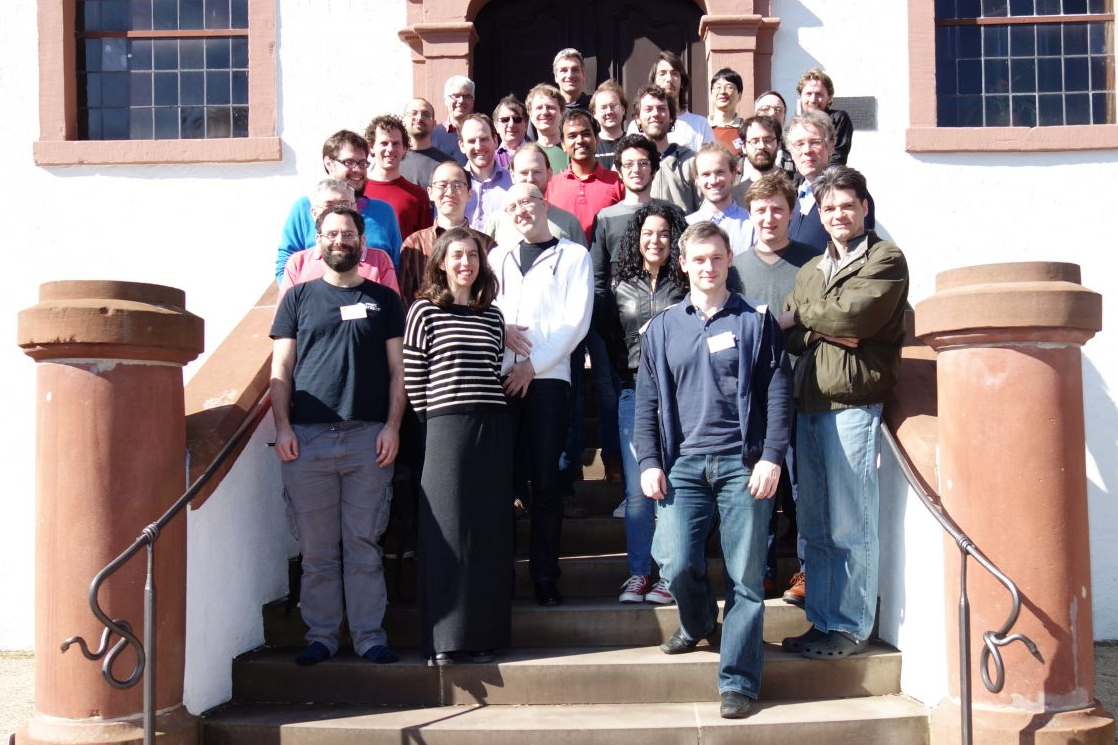
\includegraphics[width=0.85\textwidth]{16112-zoomed.jpg}
\end{center}

\vfill

\end{document}
